{
	\color{red}
\noindent
This chapter is intended to describe the technical basis on which execution
of the project depends.  The goal is to provide a detailed explanation of
the specific problem at hand, and existing work that is relevant (e.g., an
existing algorithm that you use, alternative solutions proposed, supporting
technologies).

Per the same advice in the handbook, note there is a subtly difference from
this and a full-blown literature review (or survey).  The latter might try
to capture and organise (e.g., categorise somehow) {\em all} related work,
potentially offering meta-analysis, whereas here the goal is simple to
ensure the dissertation is self-contained.  Put another way, after reading
this chapter a non-expert reader should have obtained enough background to
understand what {\em you} have done (by reading subsequent sections), then
accurately assess your work.  You might view an additional goal as giving
the reader confidence that you are able to absorb, understand and clearly
communicate highly technical material.
}

This chapter provides the technical background to the project and discusses
the relevant existing work.

\section{Genetic Algorithms}
Genetic algorithms grew from a branch of engineering which takes influence from
nature. By applying Darwinian evolutionary theory to a population of binary strings
they developed
a robust directed non-deterministic procedure to navigate search spaces with non-continuous
fitness. These search spaces are not well suited to conventional search methods
and previously were only navigatable by random walks, or bruteforce search,
and genetic algorithms provide a good general method to approach problems where
such little information is known about a space of solutions.
David Goldberg's book {\em Genetic Algorithms: In Search Optimisation \& Machine
Learning} \cite{Goldberg:1989:GAS:534133} contains a good summary of the knowledge
of genetic algorithms as it stood in the early 1990s after the vast majority of what
we know had been published.
The genetic algorithm as presented by Goldberg consists
of a repeated cycle of reproduction, crossover, and mutation; and operates on a
population of randomly seeded binary strings.

\paragraph{Reproduction}
is the mechanism by which a new population is generated. Given a fitness function
$f$ providing a measure of the quality of an individual, each member of the
population is evaluated and
assigned a score. To improve the fitness across the entire population some form
of Darwinian selection is used so that the probability of an individual
reproducing is higher for individuals with better fitness.
One such commonly chosen selection mechanism is roulette wheel (stochastic) selection.
For each individual $x$, in a population of size $n$, with fitness function $f$,
the probability of $x$ producing offspring with roulette wheel
selection is given by equation~\ref{eq:roulette}. After the reproduction
stage a new population has been created, sampled from the old.

\begin{equation}
	P(x) = \frac{f(x)}{\sum_{i=0}^{n}f(x_{i})}
	\label{eq:roulette}
\end{equation}

\paragraph{Crossover}
allows two strings in the new population to reproduce. Members of the breeding
population are paired up at random, and there is a given probability that each
pair performs crossover. For each mating pair, a number, $k$,
is selected such that $1 \leq k \leq l$, where $l$ is the population string length.
Both individuals, then swap every bit from position $k$ onwards. This stage can be
omitted for simpler evolution.

\paragraph{Mutation}
occurs after reproduction and crossover. Given a population of strings each of length
$l$, and the number of mutations expected per individual, $m$, each bit of each string
is flipped with probability $\frac{m}{l}$.

\paragraph{}
These relatively simple mechanisms provide the non-deterministic but focussed,
and surprisingly robust search procedure capable of addressing a problem when
little is known about the search space and systematically forming an answer is
unfeesable.

An interesting tagential application of FPGA technology to evolutionary algorithms comes as
a physical evolution hardware accelerator \cite{1377261}, which uses the flexibility from the
FPGA to allow incremental runtime hardware changes which allow the hardware realisation of
functions which would otherwise be impossible to construct directly in hardware.
This highlights the oportunity for aggressively efficient evolvable hardware
systems.

\subsection{Selection Mechanisms}

Goldberg et al. offer a comparison of common selection schemes for use in genetic
algorithm reproduction \cite{GOLDBERG199169}. They compared proportionate
selection, rank based selection, and tournament selection, amongst others.

\paragraph{Proportionate selection} is the set of selection mechanisms which includes
roulette wheel selection. All proportional selection schemes tie the probability of
an individual being selected for the next generation to some function of their fitness
function, $f$.

\paragraph{Rank selection} orders each member of a population by their
fitness. Then associates the probability of each individual being selected as an
individual in the next generation to their position in the ranking. This serves as
a way to "flatten" out the selection curve, and reduces the influence of
a huge spread of individual fitness.

\paragraph{Tournament selection} operates by randomly selecting a subset of the
population and the best individual from this set is chosen for further genetic
processing. Tournaments can be as small as consisting of 2 individuals, or much
larger.

\paragraph{}
There are key differences between these selection mechanisms which influences
the descision to incorporate them into an evolvable hardware platform. Proportionate
selection discriminates heavily by the fitness of inderviduals. Rank based
discriminates less and cares more about who is better (rather than by how
much they are better). Tournament selection discriminates intensley within a given
tournament but the selection process to assemble the tournament is uniformally
random, so depending on the tournament size this can be highly descriminatory
(large tournament size) or minimally descriminatory (small tournament size).
For evolvable hardware proportionate selection sees little use due to the range
of fitness values often associated with members of the population, rank and
tournament selection are used frequently.

\subsection{The Fitness Function}

\begin{equation}
	f(x) = \sum_{i=1}^{m} w_i f_i(x)
	\label{equ:multi-obj}
\end{equation}

By extending the fitness function to a weighted linear combination of a function
measuring correctness (the original fitness functon)
and any other measurements we can deploy evolutionary pressure to optimise for
additional parameters \cite{deJong:2001:RBP:2955239.2955241}. For an individual
$x$, a set of functions measuring distinct desirable aspects of individual
$\{f_1,f_2,\ldots,f_m\}$, and a set of weightings associated with each function
$\{w_1,w_2,\ldots,w_m\}$ the new fitness function $f(x)$, is given by
Equation~\ref{equ:multi-obj}.

This technique has been used to expand the success criteria for a evolvable hardware configuration
to create smaller, or more fault resistant hardware designs.

\subsection{Coevolution}

Coevolution refers to the practice of evolving to populations in tandem, this can
act as a way to divide labour (two populations solving different parts of a problem)
 \cite{Potter:2000:CCA:1108888.1108890},
or as adversaries (one population of problem proposers and another of problem solvers).
The former is used to improve the scalability of evolveable hardware to naturally
decompose the problem into subproblems.
The latter is often likened to a host/parasite or pray/predator relationship.
The framework for a coevolutionary system is only a slight extension to the
generic genetic algorithm outlined previously. In a competitive system, $P_s$ is a randomly
seeded population of problem solvers, and $P_p$ is a randomly seeded population
of problem proposers; where each individual is represented by a bitstring of
appropriate length. The fitness function of one population is inexorably tied to
the fitness function of the other.
When evaluating, each problem solver $p_s \in P_s$ is randomly associated
a problem proposer $p_p \in P_p$, and is scored based on how many problems proposed by
$p_p$ that are correctly solved. $p_p$ is scored based on how many problems
are incorrectly solved. Once each individual is scored the genetic process continues as expected,
with independent reproduction, crossover, and mutation for each population.

The evolutionary pressure on the problem proposers pushes them to be as difficult
to solve as possible, therefore emphasising problems the population of solvers
find difficult. This proves a highly effective distinguishing tool, and produces
problem proposers which create hard problems specifically tailored to the population
of problem solvers.

Extending the parallel with nature, one can modify the virulence of the parasitic
coevolutionary population. Virulence is a measure of the hostility of the aggressor.
Malaria is a highly virulent virus, often killing it's host; the evolutionary
process which drove it's development encourages causing maximum harm to the target.
An example of virus with a low virulence is the common cold, it gains nothing from
killing the host, it wants the host to survive and spread the virus; this means
there is evolutionary pressure discouraging a maximal virulence.

In some settings the population of highly virulent problem proposers develop to be much more
aggressive than the solvers can handle, meaning no solver ever manages to
successfully solve any problem, even if it could have solved some easy ones.
When individuals can no longer
differentiate themselves and push the population up the evolutionary ladder,
the coevolved populations are said to have disengaged.
By modifying the fitness function (\todo insert figure) Bullock et al. \cite{6790490}
discouraged maximally
virulent parasites. This encourages populations to stay engaged.

\section{Evolvable Hardware}

\subsection{Theory}
The foundational work in evolveable hardware is summarised by T. Higuchi et al. in their
paper {\em Evolvable Hardware with Genetic Learning} \cite{541893}. They describe
the flexibility of FPGA devices and how this can be exploited by genetic algorithms
by treating the bitstring used by the hardware for calibration as the genetic material
to be evolved. They also describe the fitness function as the total number of correct
output bits read off the hardware for all possible inputs. They succeed in evolving multiplexors and
counters but highlight a limitation of the direct evolution of the calibration
bitstring; only a subset of the bitstring include bits relevant to the function
of a specific region of the hardware. This increase in the amount of genetic
material expands the search space and extends the time required for the genetic algorithm to find a solution.
Using the proposed framework they evolve a image pattern recognition system,
and a welding robot controller which takes sensor information and traces a ditch.

\todo add graph of gate level evolution, phenotype -> genotype mapping

They highlight the need to abstract from gate level evolution to improve the
execution times of the genetic algorithm and present function level evolution
as a solution. This involves replacing gates (AND, OR, NOT, etc.) with functions
(adder, subtracter, etc.) as the atomic evolutionary components.

The capacity for evolutionary hardware to come up with bespoke and novel solutions
was explored by Adrian Thompson \cite{10.1007/3-540-63173-9_61}. A genetic algorithm
operated on a 10x10 grid of cells in the top corner of an FPGA, the aim was to evolve
a circuit capable of differentiating a high frequency input signal (10kHz) and a
low frequency input signal (1kHz). The output signal should read "high" (+5V) for one frequency
and "low" (0v) for the other. This was a truly bespoke application of evolutionary
hardware as the region exposed to the genetic algorithm had no access to any
hardware capable of timing; the differentiation task was one which the hardware
conventionally would not be able to do.

\todo include 10x10 grid schematic

The algorithm driving evolution was standard in many respects; with a population size of 50,
the most fit individual was copied verbatim into the next generation (a mechanism
called {\em elitism}), and linear rank-based selection (where the fittest
individual had a probability of selection double that of the median individual)
was used for the remaining members of the population. The probability of (single-point)
crossover occurring was 0.7 and the expected number of mutations per individual
(except the individual copied over via elitism) was 2.7. These values are in
accordance with existing research and were arrived at after domain specific
experimentation.

The 100 cell area was encoded as a string of 1800 bits. Each cell was defined
left-to-right row by row. The fitness evaluation was conducted on physical hardware
(many EHW schemes use simulations to improve training time), a series of test frequencies
were fed into the device and an single cell's output was read. The fitness of a configuration
was defined as the difference between the average output for each different input frequency
(multiplied by a constant to avoid otherwise inescapable local optimum).

After 3500 generations of evolution the genetic algorithm produced a specification
capable of distinguishing the two input signals cleanly. This is behaviour beyond
what the hardware was designed for and demonstrates the power of evolvable hardware. One of the
interesting things to come from Thompsons work was the demonstration that genetic
algorithms happily exploit undefined and strange behaviour on-chip, such as feedback
loops and more strangely; unconnected circuitry. The successful
individual's schematic was pruned of any circuitry which should not influence the
output (a direct path could not be traced from the input to the output via that route),
and the fitness of what remained {\em dropped}. The search procedure took 2-3 weeks
due to each evaluation taking up to 5 seconds.

By extending the fitness function we can apply evolutionary pressure to configurations
to nurture more than just correctness.
One of the first uses of multi-objective fitness function in evolvable hardware was
to reduce the size of the circuit \cite{785435}. Once a correct solution has been evolved the
fitness function shifts to a linear combination of correct output bits and
the number of cells innactive. This paper also introduced a mechanism for evolving the size
and shape of the underlying fabric in parallel to conventional evolvable hardware
evolution, this allows for a system to define
how large it should be.

Evolving the size and shape of the circuitry involves defining how mutation and recombination
of circuit size operates. The mutation step alters the number of rows and columns of a circuit
with equal probability, and new cells are initialised randomly. Recombination is a
mechanism for crossover of non-uniform circuit sizes which involves exchanging cells
and way to preserve positional connections of cells in the case that the new circuit
is too restrictive for direct copying.
Both multi-objective fitness functions and evolved circuit structure
apply evolutionary pressure to improving the quality of evolutionary hardware
beyond simple performance accuracy.

An alternative substrate for evolvable hardware to FPGAs comes in the form of field
programmable transistor arrays (FPTAs) \cite{869347}. These offer similar functionality
to FPGAs, but where FPGAs allow gate-level flexibility, FPTAs allow a user to specify
the placement and configuration of transistors. Evolutionary hardware operating on this
level is subject to worse scaling issues than gate-level evolvable hardware, but has a
great deal more flexibility.

One of the largest problems with evolvable hardware is how the system scales as the
circuit function increases. The poor scaling of the genetic algorithm is due to two
features; the larger circuit size required (and the consequently larger genetic material),
and the larger number of test-cases in the evaluation function. One way to combat this
involves decomposing the problem into subsystems \cite{10.1007/978-3-540-46239-2_5}.
This reduced granularity reduces the search space of solutions and improves search
performance at the cost of reduced flexibility to construct novel circuitry.

A similar method proposed by J. Torrensen suggests allowing the evolutionary
process itself to subdivide the process, increased complexity evolution \cite{Torresen2002}. The area
of an FPGA is divided into subsets of cells and the function of each of these
subsets is decided manually or by the evolutionary process.
The first system, dubbed "partitioned training vectors" involves feeding the
complete input information individually to each subset, but only reading off
a subset of the output bits from each region of cells. In this way each subset
can distinguish a few answers perfectly and the other input combinations are
identified by another group of cells.
A parallel is drawn
with artificial neural nets where evolution is applied to the connections between
these subsets, and each subset evolves it's functionality locally. To demonstrate
the efficiency of such a system using the vector approach a character detection system was evolved, capable
of classifying images of letters of size 5 by 6 pixels, the number of generations
required to train the classifier dropped substantially as the number of allowed subsystems
increased. More success was found applying this technique to a prosthetic hand controller
which achieved better performance than the artificial neural net equivalent.

\todo insert image of "partitioned training vectors" and "partitioned training sets" from "A scalable approach to evolvable hardware"

These methods all deal with reducing the search space or dividing the problem into
more manageable workloads. The problem remains with the scaling inefficiency in
regards to the number of test cases to be applied to a circuit during evaluation.

This other, less explored facet of the scaling issues appears in the form of the number of
evaluations required to calculate the fitness function. For evolved circuitry
with $n$ input bits, the fitness function requires $O(2^{n})$ time to evaluate;
for example, a 2-bit adder requires evaluation against all 16 ($2^{2 \cdot 2}$) possible combinations
of 2 2-bit numbers, whereas for a 3-bit adder this value grows to 64 ($2^{2 \cdot 3}$).
For practical evolution of larger circuits this requires some careful thought.

\todo Generalized Disjunction Decomposition for Evolvable Hardware \cite{1703646}
Addresses scaling issue, offers a new type of decomposition strategy.

\todo Evolved Digital Circuits and Genome Complexity \cite{1508485}
Improving scaling issue my investigating genotypic complexity, also considers shrinking search space

\todo Extrinsic vs intrinsic evolution

\subsection{Application}

Part of the charm of evolutionary hardware is it's vast capacity for strange
solutions
to problems. The nature of a simple fitness function driving the evolutionary
process means that any point in the search space which performs perfectly is
equally weighted as any other point in the search space.

Nowhere is this more apparent than with the antennas featured on NASA's ST5 mission
which were designed by genetic algorithms \cite{Antenna}. Although
this is a slight departure from the circuit design applications mentioned thus
far it is a fantastic example of the strengths of evolution derived design.
Traditional (human-driven) antenna design is a laborious process requiring
seasoned professionals with a great deal of experience in the area. By creating
a fitness function which outlined the design requirements of the device, and
tuning a suitable genetic algorithm, huge portions of the design process can
be automated.

Figure~\ref{fig:antenna} features the evolved antenna design which
saw use in space. Clearly it is a novel design, looking like an art piece
more at home in the Tate Modern than a piece of space-grade equipment, and such
designs are typical of evolved systems. The antenna performed successfully
throughout the operational lifetime of the spacecraft. This avenue of design
provided completely fresh ideas, unburdened by the prejudice of previous
success. The antenna achieved a larger range of detection angles than the
hand designed counterpart and required only 3 person-months of work to set up and
monitor the evolutionary process rather than the 5 person-months of work which
would otherwise be required.

\begin{figure}
	\centering
	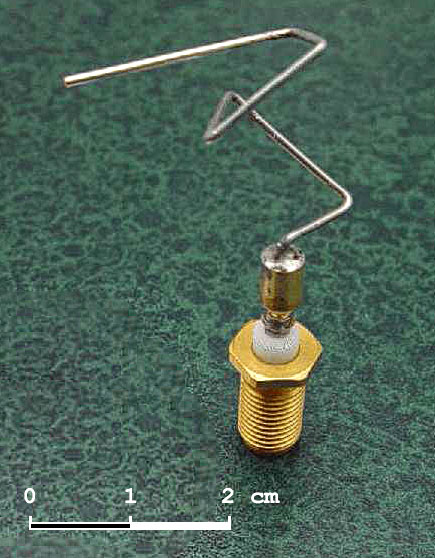
\includegraphics[height=5cm]{NASA_antenna.jpg}
	\caption{NASA evolved antenna \cite{Antenna}}
	\label{fig:antenna}
\end{figure}

The list of evolutionary hardware successes is long.

\todo Evolutionary hardware design \cite{Sekanina}
talk about case studies, logic synthesis \cite{Vasicek2011}, image filter evolution

\todo Hybrid Evolvable Hardware for automatic generation of image filters \cite{HybridFilter}
Architecture for fast image filters - no need to use a bitstream to reprogram

A series of general purpose evolvable hardware chips have been developed for
applications ranging from telecommunications circuits to robot controllers.
Using tournament selection and elitism T. Higuchi et al. created a sensor
driven robot controller, and developed an EHW chip capable of lossless image
compression outperforming existing standards. All this was performed on off
the shelf, components designed to accelerate the evolvable hardware process
for gate-level evolution \cite{HiguchiRW}. A similar success story with hardware
designed for evolution takes the form of a prosthetic hand controller with
a training time of only 10 minutes to adapt to a new user \cite{Kajitani1999AnEH}.

\todo Phylogeny, Ontogeny, and Epigenesis: Three Sources of Biological Inspiration for Softening Hardware

\todo POEtic Tissue: An Integrated Architecture for Bio-Inspired Hardware

\todo Routine duplication of post-2000 patented inventions by means of genetic programming

\todo Toward automated design of industrial-strength analog circuits by means of genetic programming

\todo Challenges of evolvable hardware: Past present and the path to a promising future \cite{Haddow2011}

\todo MEH: Modular Evolvable Hardware for designing complex circuits

\subsection{Arithmetic Circuits}

\todo MULTIPLE-VALUED COMBINATIONAL CIRCUITS SYNTHESISED USING EVOLVABLE HARDWARE APPROACH
Genetic programing to add numbers via gate trees

\todo Synthesis of Adder Circuit Using Cartesian Genetic Programming

\todo Scalability problems of digital circuit evolution evolvability and efficient designs

\section{Dynamic Problems}
\todo A little spiel about what dynamic are and why they are relevant

\todo A self-organizing random immigrants genetic algorithm for dynamic optimization problems \cite{1703646}
Improves diversity and escaping from local optima, dynamic optimisation problem

\todo A Genetic Algorithm Approach to Dynamic Job Shop Scheduling Problem. \cite{Lin1997AGA}
Different sort of dynamic problem - varying input, constant fitness criteria

\todo Designing evolutionary algorithms for dynamic optimization problems\cite{Branke2003}

\subsection{Fault Tolerance}
\todo Understanding inherent qualities of evolved circuits: Evolutionary history as a predictor of fault tolerance

Fault tolerance in regards to hardware design is defined as a systems capacity to
remain functional despite component failure. This is usually in reference to
post-fabrication faults which affect can effect chip yields, but evolutionary
hardware also looks extensively into faults which occur some way into the
operational lifespan of a product; this can be component failures do to environmental
conditions or an aging device.

Genetic algorithms by their nature produce designs which are resilient in the face
of change. More fragile designs are often mutated into obscurity whereas ones with
natural fault tolerance endure. Amplifying the effects of this subtle pressure towards fault
tolerant design is a mainstay of applied evolutionary hardware research.

\todo Evolvable Hardware and its application to pattern recognition and fault-tolerant systems\cite{10.1007/3-540-61093-6_6}
learning an XOR circuit, discussion of 2 applications: pattern recognition, ditch tracer

\todo Evolutionary techniques for fault Tolerance\cite{651463}
Fault tolerant fitness function, fault tolerance by natural process, control for a robot evolved

\todo On the Automatic Design of Robust Electronics Through Artificial Evolution
Addresses problems of EHW only working at certain temperatures. Selection pressure
for robustness added by executing fitness evaluation and different temperatures

One of the potential problems with fitness function driven exploration comes in
the form of environment specific effects. Somefolk et al. explored the problem
where the evolutionary process honed in to a solution which exploited temperature
sensitive behaviours of a chip \cite{10.1007/BFb0057603}.

By defining a list of the faults a device is expected to encounter during it's
lifespan one can design a fitness function which tests a given circuit under
normal conditions and faulty conditions \cite{Keymeulen2000}. This technique applies explicit
evolutionary pressure to find designs which can tolerate a specific set of
known and understood faults. Alongside the proposed fitness driven fault mitigation
approach \cite{Keymeulen2000} introduces an alternative mechanism which takes the
highest performing individual in a fault-free system and explores the performance
of mutants generated from it in a fault environment, this emphasises the natural
fault tolerant properties of genetic algorithms. In some situations the mutants
could not recover from the injected fault, in these cases the genetic algorithm
was to restart and continue searching through the design space under the conditions
of the fault.

Using conventional genetic algorithm, along with tournament selection, and elitism
J. Lohn et al. demonstrate the capacity
of evolvable hardware to reduce the impact of "stuck at zero" faults \cite{10.1007/3-540-36553-2_5}. They
conducted their experiments on a simulated FPGA, attempting to evolve a quadrature
decoder, a device which indicates
the direction of rotation of a wheel. The system was evolved in the presence
of the fault and was capable of operating perfectly despite it.

\todo Addressing the Metric Challenge: Evolved versus Traditional Fault Tolerant Circuits\cite{4291951}
Compairson peice

\todo Evolviving Redundant Structures for Reliable Circuits\cite{4291954}
Novel redundancy structures, challenge to tune evolution to find these novel structures

\todo Evolving Variability-Tolerant CMOS Designs\cite{10.1007/978-3-540-85857-7_27}
High failure rate in CMOS designs, GA vs CGP, unconventional designs with variability-tolerance

\todo Implementation of a Power-aware Dynamic Fault Tolerant Mechanism on the Ubichip Platform\cite{10.1007/978-3-642-15323-5_26}
Built in self repair (BISR), dynamic fault tolerant system on the Ubichip platform

\todo Machine Learing-based Anomaly Detection for Post-silicon Bug Diagnosis\cite{6513558}
Post-fab bug detection with ML

\todo Self-healing router architecture for reliable network-on-chips\cite{8292030}
Redundancy based, rerouting

The space industry naturally wants to emphasise longevity in their design goals,
this was a clear desire with the NASA's CT5 mission, and as previously mentioned
the genetic algorithm devised antenna performed to the highest standards until the
end of the missions lifespan \cite{Antenna}.

Circuitry hosted in space is subject to a breadth of extreme conditions; temperature
drifts, radiation, and poor serviceability to name a few. Radiation is a particular
issue, bombarding electronics with electrons and protons causes huge damage.

Space technology has traditionally used radiation-hard materials to achieve
radiation resistance. These materials resist the ionising effects of radiation
and reduce the probability of radiation-induced silicon faults. These materials
are expensive and definitely not the only way to create long-life deep space
electronics. A. Sotica et al. propose using genetic algorithms to drive
in-situ hardware reconfiguration to bypass faulty areas \cite{1331112}. Experiments
were performed on an FTPA with evolution controlled by an external stand-alone
board-level evolvable system (SABLES) capable of performing an evaluation in 2ms.

In experiments bombarding the chip with upto 350krad the system was usually able
to recover functionality, and there were significant performance improvements over
the unevolved comparison chip.

\todo Design of self-repairing control circuit for brushless DC motor based on evolvable hardware\cite{8046381}
Radiation space damage, dynamic partial reconfiguration

\todo Towards evolving fault tolerant biologically inspired hardware using evolutionary algorithms

\todo Intelligent Fault Tolerance techniques

\todo Requirement for extensive fault models to accurately inject faults

Fault tolerance in conventional hardware design requires redundancy in some
form. Predictive preemptive instruction rescheduling on a different processor
core \cite{Soman} uses multi-core redundancy to mitigate the cost of faulty instruction
execution. Cross-core redundancy is used by core salvaging \cite{Powell} which shares execution
pipeline resources between cores, in order to reroute execution pipelines
around faulty components. This is similar in principal to StageWeb \cite{StageWeb}, which also
features pipeline rerouting but with an emphasis in scaling flexibility.

This is a very different approach to evolvable hardware centric fault
tolerance which exploits flexibility. Many of the aforementioned modern
fault techniques do little to improve the performance of faulty architectural
processor components and rely on the ability to route around them.

\subsection{Dynamic Optimisation}
It has been well established that flexible systems can provide huge boosts to,
not only circuit efficiency, but also performance.

\todo Configurable memory systems for embedded many-core processors\cite{DBLP:journals/corr/BatesCM16}
\todo FPGA deep learning accelerators
